\begin{frame}

Part 1:
\vspace{0.2cm}

{\LARGE \textbf{\textcolor{blue}{Abstract Domain}}}

\end{frame}


\begin{frame}[fragile]{\textcolor{blue}{Application Interface}}

\begin{minipage}{0.5\textwidth}
\begin{center}
\begin{tikzpicture}[thick,scale=0.8, every node/.style={transform shape}]

\umlclass[fill=red!20
%,y=+3
,y=+5, x=-6.5
]{VSAResult}{
}{ 
is\_reachable(basic\_block) : bool \\
is\_resultat\_available(bb, value) : bool \\
get\_abstract\_value() : VSAResultValue \\
}

\umlclass[fill=red!20
%,y=+3
,y=1.5, x=-6.5
]{VSAResultValue}{
}{ 
test(predicate, constant) : tristate \\
min() : int \\
max() : int \\
size() : int \\
consant() : int \\
is\_constant() : bool \\
}

\end{tikzpicture}
\end{center}
\end{minipage}
\begin{minipage}{0.49\textwidth}
\begin{itemize}
\item after a successful pass:\\
\quad {\color{blue} auto\& res = vsap.get\_result();}
\item query information related to \\basic block (reachable or not) and/or variable (abstract value)\\
%\quad {\color{blue} auto\& res = vsap.get\_result();}
\end{itemize}
\end{minipage}

\end{frame}

\begin{frame}[fragile]{\textcolor{blue}{Background to LLVM Integer Types}}
\begin{itemize}
\item In LLVM the type of $N$-bit integers is the set $\{0,1\}^N, \text{for~} N \in \{1,\dots, 2^{23}-1\}$.
\item In the in-memory-representation, these types are represented by the LLVM class APInt.
\item This type is used for both signed and unsigned integers.
 
\item We use APInt 	 in our implementation of abstract domains.

\end{itemize}

\end{frame}

\begin{frame}[fragile]{\textcolor{blue}{LLVM Integer Operations}}
\begin{large}Arithmetic Operations:\end{large} \\
In LLVM there are separate $\texttt{div}$ and $\texttt{rem}$ operations for signed and unsigned integers. 
For $\texttt{add}$, $\texttt{sub}$ and $\texttt{mul}$, there is no such distinction needed.
\begin{itemize}
\item $\texttt{<result> = add [nuw] [nsw] <bitWidth> <op1> <op2>}$
\item $\texttt{<result> = sub [nuw] [nsw] <bitWidth> <op1> <op2>}$
\item $\texttt{<result> = mul [nuw] [nsw] <bitWidth> <op1> <op2>}$
\item $\texttt{<result> = udiv [exact] <bitWidth> <op1> <op2>}$ 
\footnote{\label{not-impl} $\texttt{exact}$-flag not used in our implementation.}
\item $\texttt{<result> = sdiv [exact] <bitWidth> <op1> <op2>} ^{~\ref{not-impl}}$
\item $\texttt{<result> = urem <bitWidth> <op1> <op2>}$
\item $\texttt{<result> = srem <bitWidth> <op1> <op2>}$
\end{itemize}

\end{frame}

\begin{frame}[fragile]{\textcolor{blue}{LLVM Integer Operations, Continued}}
Bitwise Operations:
\begin{itemize}
\item $\texttt{<result> = shl [nuw] [nsw] <bitWidth> <op1> <op2>}$
\item $\texttt{<result> = lshr [exact] <bitWidth> <op1> <op2>}$ \footnote{\label{not-impl2} $\texttt{exact}$-flag not used in our implementation.}
\item $\texttt{<result> = ashr [exact] <bitWidth> <op1> <op2>}^{~\ref{not-impl2}}$
\item $\texttt{<result> = and <bitWidth> <op1> <op2>}$
\item $\texttt{<result> = or <bitWidth> <op1> <op2>}$
\item $\texttt{<result> = xor <bitWidth> <op1> <op2>}$
\end{itemize}

\end{frame}

\begin{frame}[fragile]{\textcolor{blue}{Bounded Set}}
\begin{itemize}
\item A bounded set represents sets of values upto a given cardinality $k$ or $\top$: \\
$\mathrm{BS}_{N} \coloneqq \{M\in \mathcal{P}(\texttt{i}N)\mid |M| \leq k\} \dot\cup \{ \top \}$ \\
\item $\sqcup$ and $\sqsubseteq$ on bounded sets essentially reduce to $\cup$ and $\subseteq$ on sets.
\item Any set with more elements than $k$ are represented by $\top$.
\end{itemize}

\end{frame}

\begin{frame}

\end{frame}

\begin{frame}[fragile]{\textcolor{blue}{Abstract Domain Class Structure}}

\begin{center}
\begin{tikzpicture}[thick,scale=0.8, every node/.style={transform shape}]

\umlinterface[]{AbstractDomain}{
}{ 
add(other) : AbstractDomain \\ /* other arithmetic and logical operations */ \\ \\

icmp(other, predicate) : (AbstractDomain, AbstractDomain) \\ \\
leastUpperBound(other) : AbstractDomain \\ 
lessOrEqual(other) : bool \\
}

\umlclass[x=-3.5,y=-4.0]{CompositeDomain}{}{upgrade() : void}
\umlclass[x=+2.5,y=-4.0]{BoundedSet}{
values : set$<$APInt$>$
isTop : bool}{}
\umlclass[x=+3.0,y=-6.0]{StridedInterval}{
min, max, stride : APInt \\
isBottom : bool}{}


%\umlclass[x=-3,y=-6.5]{OperationNDim$<$vec$>$}{}{}

%\umlclass[x=3,y=-6.5]{OperationNDim$<$novec$>$}{}{}

\umlinherit[geometry=|-]{CompositeDomain}{AbstractDomain}
\umlinherit[anchor1=north,anchor2=-41]{BoundedSet}{AbstractDomain}
\umlinherit[geometry=-|-, arm1=0.5cm,anchors=east and east]{StridedInterval}{AbstractDomain}
%\umlaggreg[]{OperationNDim$<$T;U;V$>$}{OperationMass}
%\umlaggreg[]{OperationNDim$<$T;U;V$>$}{OperationConvection}
\umlaggreg[]{CompositeDomain}{BoundedSet}
\umlaggreg[geometry=-|-,anchors=east and west]{CompositeDomain}{StridedInterval}


\end{tikzpicture}
\end{center}

\end{frame}

\begin{frame}[fragile]{\textcolor{blue}{Connection of the Results to the Internal Abstract Domain}}

\begin{center}
\begin{tikzpicture}[thick,scale=0.8, every node/.style={transform shape}]

\umlinterface[]{AbstractDomain}{
}{ 
add(other) : void\\ /* other methods */ \\ \\
leastUpperBound(other) : void \\ 
lessOrEqual(other) : bool \\
}

\umlclass[x=-3.5,y=-3.5]{CompositeDomain}{}{upgrade() : void}
\umlclass[x=+2.0,y=-3.5]{BoundedSet}{values : set$<$int$>$}{}
\umlclass[x=+2.0,y=-5.5]{StridedInterval}{min, max, stride : int}{}

\umlclass[fill=red!20
%,y=+3
,y=0.5, x=-6.5
]{VSAResultValue}{
}{ 
test(predicate, constant) : bool \\
min() : int \\
max() : int \\
size() : int \\
consant() : int \\
is\_constant() : bool \\
}

%\umlclass[x=-3,y=-6.5]{OperationNDim$<$vec$>$}{}{}

%\umlclass[x=3,y=-6.5]{OperationNDim$<$novec$>$}{}{}

\umlinherit[geometry=|-]{CompositeDomain}{AbstractDomain}
\umlinherit[anchor1=north,anchor2=-42]{BoundedSet}{AbstractDomain}
\umlinherit[geometry=-|-, arm1=0.5cm,anchors=east and east]{StridedInterval}{AbstractDomain}
%\umlaggreg[]{OperationNDim$<$T;U;V$>$}{OperationMass}
%\umlaggreg[]{OperationNDim$<$T;U;V$>$}{OperationConvection}
\umlaggreg[]{CompositeDomain}{BoundedSet}
\umlaggreg[geometry=-|-,anchors=east and west]{CompositeDomain}{StridedInterval}

\umlaggreg[geometry=|-|,anchor1=north,anchor2=north,arm1=0.5cm]{VSAResultValue}{AbstractDomain}

\end{tikzpicture}
\end{center}

\end{frame}